\section{Trajectory analysis} \label{ch:trajectory}

**intro**

\subsection{Governing equations}\label{sec:gov}

\begin{wrapfigure}{r}{0.4\textwidth}
		\centering
		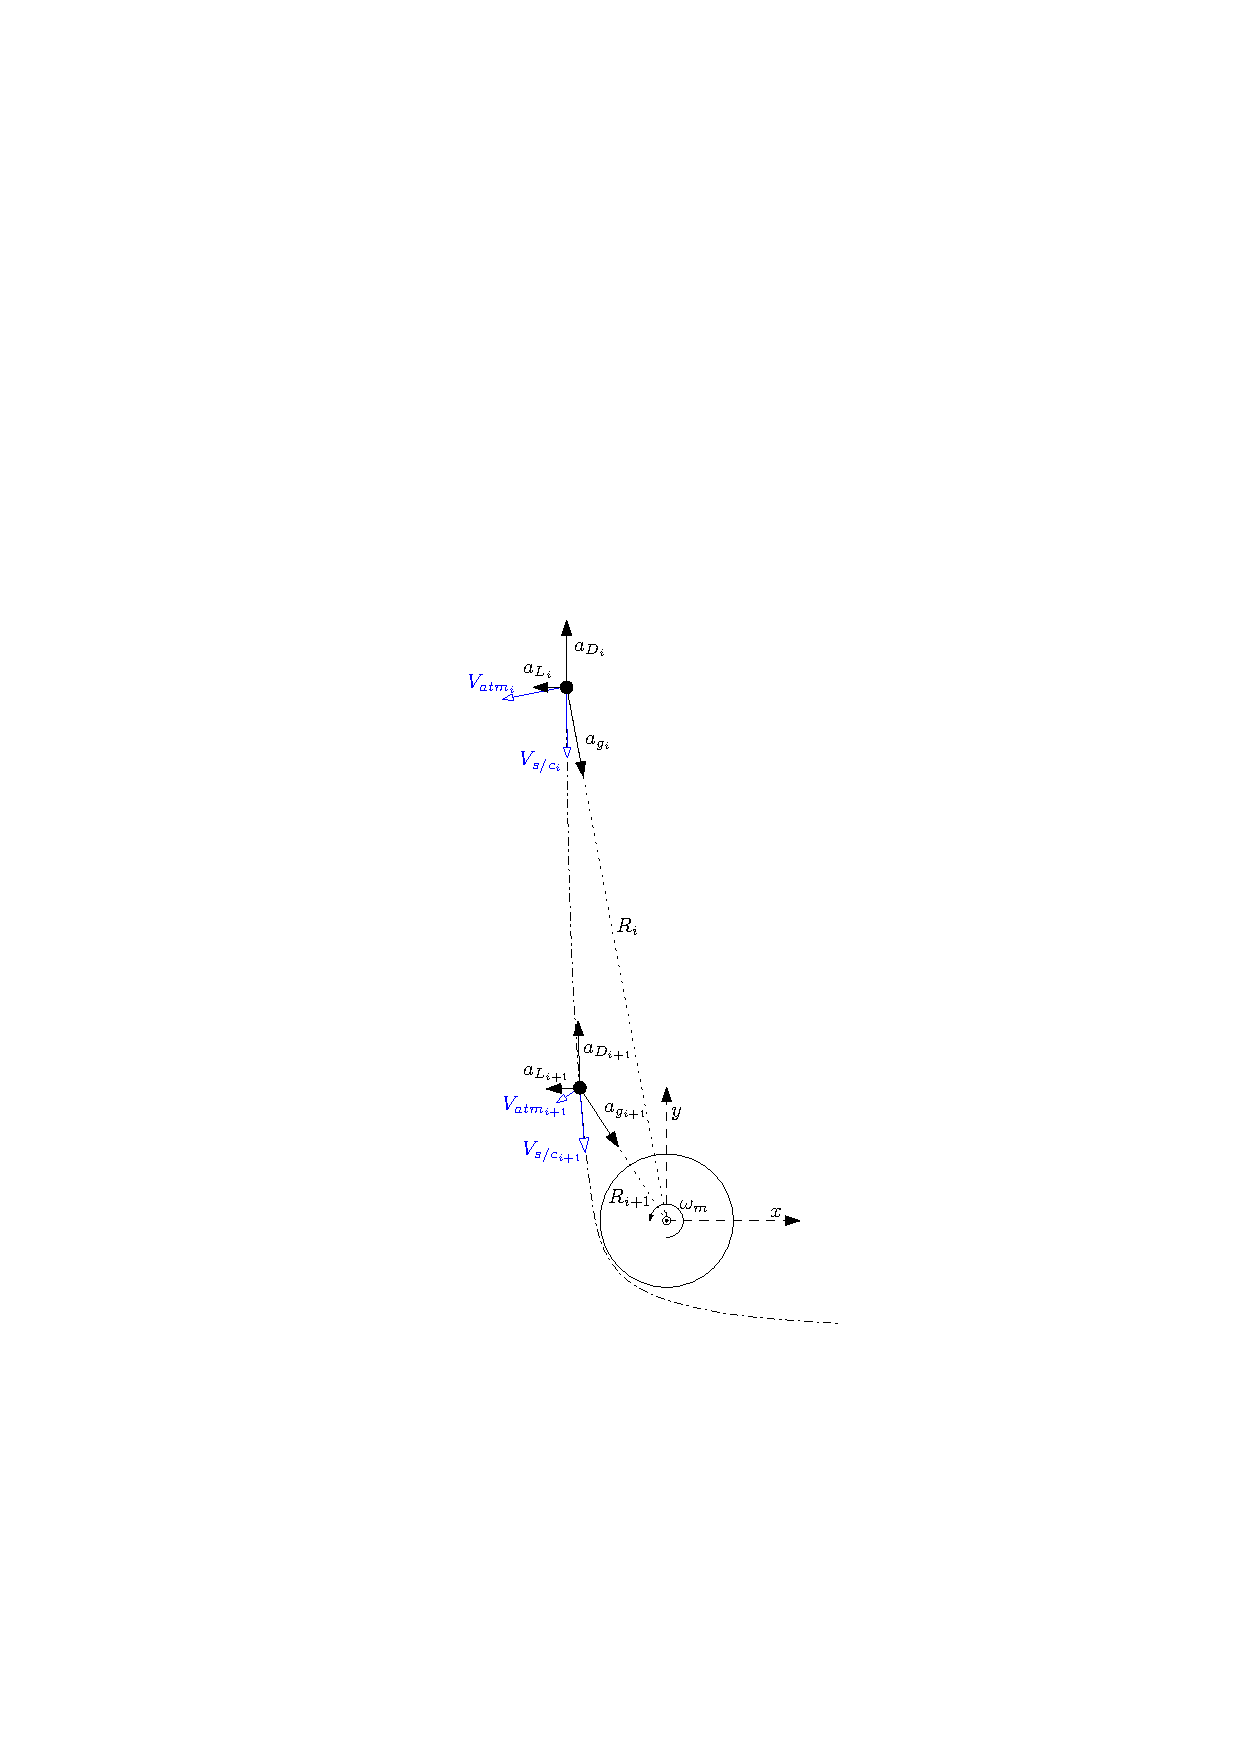
\includegraphics[width = 0.4\textwidth]{Figure/orbital_mechanics.pdf}
		\caption{The kinetic diagram visualizing the governing equations of the trajectory analysis}
		\label{fig:orb}
\end{wrapfigure}

The motion of a spacecraft can be broken down in some dominant contributors. These contributors are the gravitational pull and the aerodynamic forces. Disturbances like solar radiation or gravitational pull from moons or other bodies is neglected in the model.

To be able to fully describe the contributors, two reference frames need to be defined. The non rotating inertial frame is defined with its origin in the centre of mass of Mars if it would be perfectly spherical, this is the \gls{mci}. 
Another reference frame is the \gls{mcmf}. in our first model the origin and the z-axis of both reference frames is equal (so no axis tilt is taken into account). The difference between the two is that the \gls{mcmf} is rotating around the z-axis with rotational velocity \gls{con:omegamars} compared to the \gls{mci}.

The gravitational pull is described by Newtons law of gravitation, together with Newton's second law, it can be written as an acceleration as in equation \ref{eq:nG}.

\begin{equation} \label{eq:nG}
\gls{sym:g} = -\frac{\gls{con:G}\gls{con:Mmars}}
					{\gls{sym:R}^3}\gls{sym:Rv}
\end{equation}

The aerodynamic forces are described by the lift and the drag, these forces are acting in the direction and orthogonal to the velocity of the spacecraft with respect to the atmosphere, this is the velocity of the spacecraft in the \gls{mcmf}. To make be able to express the aerodynamic forces in the \gls{mci} this velocity needs to be converted to \gls{mci} as in equation \ref{eq:Vsc_mcmf_mci}.

\begin{equation} \label{eq:Vsc_mcmf_mci}
\left.\gls{sym:Vvsc}\right|_{MCMF}^{MCI} = \gls{sym:Vvsc}_{,a} = \left.\gls{sym:Vvsc}\right|_{MCI} - \left(\gls{con:Omegamars} \times \gls{sym:Rv} \right)
\end{equation}

The aerodynamic accelerations due to the lift and the drag are described by equations \ref{eq:aL} and \ref{eq:aD} respectively.

\begin{equation} \label{eq:aL}
\gls{sym:aL} = \frac{\gls{sym:CL}\gls{sym:rho}\gls{sym:A}}{2 \gls{sym:m}} 
				\left|\gls{sym:Vvsc}_{,a}\right|^2
				\frac{\gls{sym:Vvsc}_{,a} \times \mathbf{z}}
				{\left| \gls{sym:Vvsc}_{,a} \times \mathbf{z}\right|}
\end{equation}

\begin{equation} \label{eq:aD}
\gls{sym:aD} = \frac{\gls{sym:CD}\gls{sym:rho}\gls{sym:A}}{2 \gls{sym:m}}
				\left|\gls{sym:Vvsc}_{,a}\right|^2 \frac{\gls{sym:Vvsc}_{,a}}{\left|\gls{sym:Vvsc}_{,a}\right|}
\end{equation}

\subsection{Program structure}\label{sec:prog_struct}

In order to use the governing equations (equation \ref{eq:final}**!!need label!!**) to produce usefull results they have to be implemented in a simulation which calculates the trajectory. From this calculated trajectory the program has to extract usefull data and conclusions. To model aerodynamic forces on the spacecraft an atmosphere model is needed. The atmosphere model used is presented in subsection \label{subsec:atmos}. The three different modules comprising the program are discribed in subsection \ref{subsec:modules}. In subsection \ref{subsec:flow} a flowchart of the program is presented.

\subsubsection{Atmosphere model}\label{subsec:atmos}
As stated in Section \ref{sec:control}, for the atmospheric model the NASA software \gls{marsgram} is used. The atmospheric properties are queried at equally spaced points: at all latitudes and longitudes at an interval of $10 [degrees]$, and heights from $0$ to $400 [km]$ at an interval of $5 [km]$. The software generates data based on equations for atmosphere properties and incorporates the high amount of dust on Mars, which has a big effect on the absorbed radiation heat from the sun. The output of the program is, among others, the density, temperature and gas composition at that query point, along with other less important parameters. \cite{Justus2001}
This data is then saved for processing during trajectory simulation. In the trajectory simulation software, the atmospheric properties at certain points in the atmosphere are required. The discrete atmosphere data is thus interpolated to obtain an estimate of there properties. 

\subsubsection{Modules} \label{subsec:modules}

The program first implements the governing equations on each time step. Secondly two modules were created, one to find feasible orbits and another to calculate the full orbit of the orbits which are found to be feasible. These three modules are described below.

\paragraph{Implementation of governing equations}\textit{orbit.m}

The module implementing the governing equations has a lot of input data of which most are constants and vehicle parameters. One of the inputs is the dataset created by the atmospheric model described in subsection \ref{subsec:atmos}. The density and gravitational acceleration taken from this dataset is different for each cycle of the program and dependent on the height, longitude and latitude of the spacecraft. Also the previous location, velocity and acceleration (in vector form) are constantly changing inputs.

The input variables are directly filled in into equation \ref{eq:final}. This creates output values for the location, velocity and acceleration. Both the total acceleration and the separate accelerations due to the drag, lift and gravitation are outputted.
\paragraph{Orbit selection} \textit{orbit\_selection.m}

**input

In the module for orbit selection first the initial conditions are created. One of the initial conditions is that the entry velocity is $7 \frac{km}{s}$. After this initialization \textit{orbit.m} is called for each time step. After each time step the data is analyzed and three conditions are filled in. The condition \textit{inatmos} is true when the spacecraft has ever been inside the atmosphere of mars. The condition \textit{crash} is true when the spacecraft touches the surface of mars in the first entry into the atmosphere. Finally the condition \textit{inorbit} is true when the spacecraft either leaves the atmosphere with a velocity smaller than the escape velocity at that point or when the spacecraft did never enter the atmosphere and the velocity at the point the simulation is terminated is smaller than the escape velocity at that point. The values of these conditions is used in \textit{orbitcheck.m} to determine the feasible initial conditions.

**output

\paragraph{Full orbit simulation} \textit{orbit\_full.m}

**

\paragraph{Run orbit selection} \textit{orbitcheck.m}

**

\subsubsection{Flowchart} \label{subsec:flow}
**flowchart

\begin{figure}[H]
\centering
\hspace{-23mm}
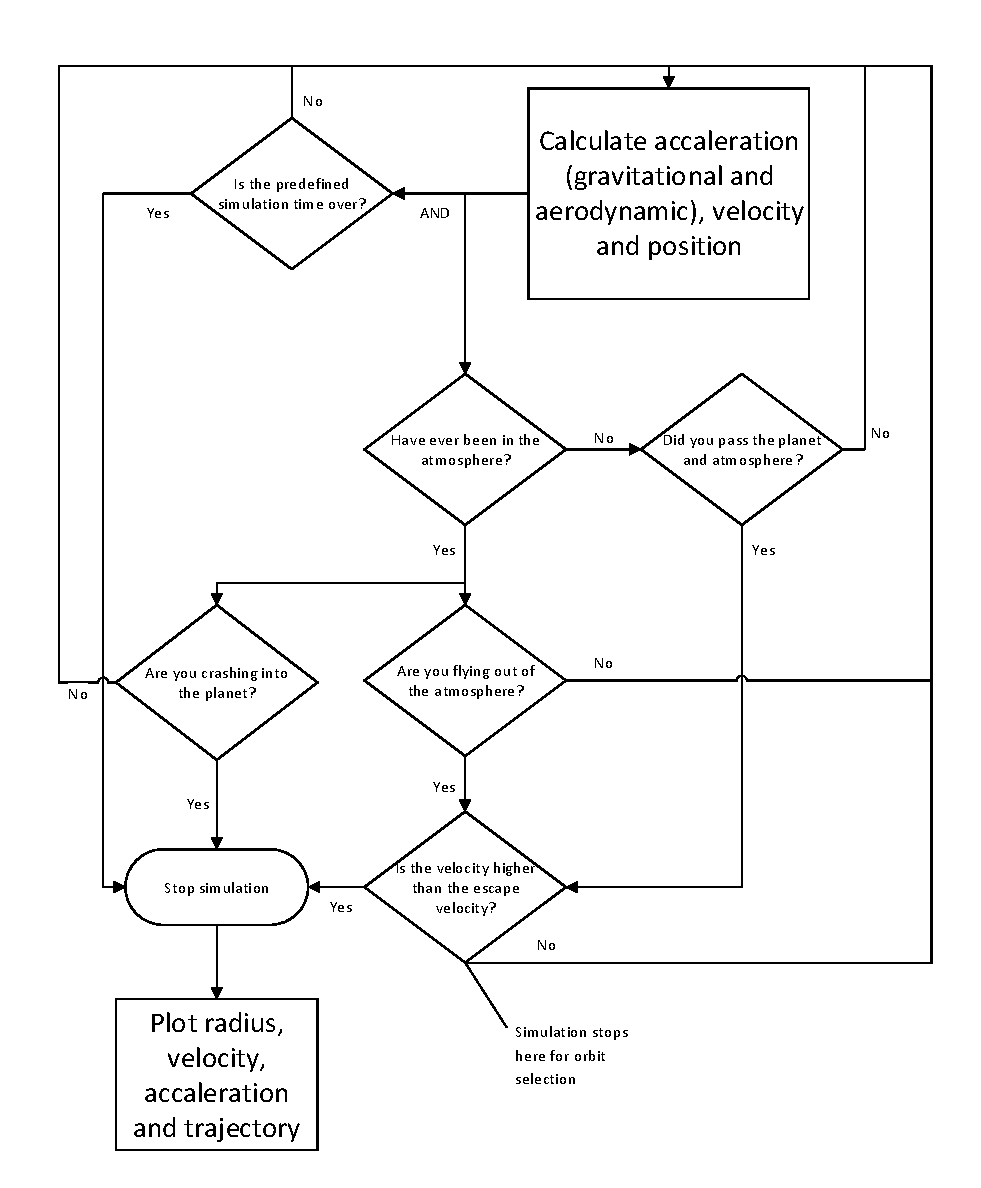
\includegraphics[width = 0.8\textwidth]{Figure/astro_tool.pdf}
\vspace{-5mm}
\caption{Flowchart of the working principle of the trajectory analysis program}
\label{fig:traj_flow}
\end{figure}

\subsection{Verification and validation}